%%]dvipdfm
\expandafter\def\csname CTEX@spaceChar\endcsname{\hspace{1em}}
\documentclass[master]{NJUthesis}
%\documentclass[twoside, master]{NJUthesis}
% 可选参数:
%   review 审阅模式,激活后个人、导师与学校信息均被隐去
%   oneside/twoside 单面/双面打印
%   phd/master 博士/硕士论文
% 下面三个选一个:
% dvi2pdf 使用 dvi2pdf(x) 生成最终的 PDF 文档 (缺省设置,不建议修改)
% dvips 使用 dvips 生成最终的 PS 文档
% pdftex 使用 pdfLaTeX 生成最终的 PDF 文档

%%%%%%%%%%%%%%%%%%%%%%%%%%%%%%
%% 导言区
%%%%%%%%%%%%%%%%%%%%%%%%%%%%%%

% 小节标题靠左对齐
\CTEXsetup[format+={\flushleft}]{section}

% 设置链接颜色
\hypersetup{
% pdf 属性
            pdftitle={LaTeX Thesis Template of Nanjing University}, %
            pdfauthor={San Zhang}
}

% 表格
\usepackage{longtable, multirow}
% 英文使用 Times 字体
\usepackage{times}
% 源代码
\usepackage{fancyvrb}
% 自定义列表样式
\usepackage{enumitem}
\usepackage{url}
\usepackage{amsmath}
\usepackage{amssymb}
\usepackage{moreverb}
\usepackage{txfonts}
\usepackage{mathcomp}
\usepackage{graphicx}
\usepackage{subfigure}
\usepackage[linesnumbered,boxed,ruled,vlined]{algorithm2e}
\usepackage{array}
\usepackage{multirow}

%%	added by Jiang
\usepackage{extarrows}	%使用长箭头
\usepackage{nomencl}	%与术语表有关的包
\usepackage{booktabs}
\usepackage{ccmap}

%% added by lhy
%%取消默认楷书命令
\let\kaishu\relax 
%% 配置新的楷书命令,粗体用方正粗楷简体,普通用方正楷体简体
%% 这里其实是可选的,如果有什么更合适的楷体字体,可以自行替换
\setCJKfamilyfont { bfkt }[BoldFont=FZCKJT.ttf]{FZKTJT.ttf}
%% 添加新的字体命令kaishu,中文用方正楷体,英文用times
\NewDocumentCommand \kaishu { } { \CJKfamily { bfkt } \fontspec{Times New Roman}}
%% 全文所有英文默认使用Times英文字体
\setmainfont{Times New Roman}

\makenomenclature

\setcounter{topnumber}{5}

\theoremstyle{plain}
\newtheorem{definition}{\hspace{2em}定义}[chapter]
\newtheorem{lemma}{\hspace{2em}引理}[chapter]
\newtheorem{theorem}{\hspace{2em}定理}[chapter]
\newtheorem{property}{\hspace{2em}性质}[chapter]
\newtheorem{example}{\hspace{2em}例}[chapter]
\newtheorem{myrule}{\hspace{2em}规则}[chapter]


\newcommand{\tabincell}[2]{\begin{tabular}{@{}#1@{}}#2\end{tabular}}% 表格内换行
\renewcommand{\footnoterule}{%脚注线
  \kern -3pt
  \hrule width 2.3in height 0.4pt
  \kern 2pt
}


\begin{document}

%%%%%%%%%%%%%%%%%%%%%%%%%%%%%%
%% 封面部分
%%%%%%%%%%%%%%%%%%%%%%%%%%%%%%

% 国家图书馆封面内容字符串
% 仅博士需要填写并保证模板参数选择了 phd
\classification{}
\confidential{}
\UDC{}
\titlelinea{南京大学学位论文}
\titlelineb{~\LaTeX{}~模板}
\titlelinec{}
\advisorinfo{南京大学~软件学院}
\chairman{XXX 教授}
\reviewera{某某某某 副研究员}
\reviewerb{XXX 教授}
\reviewerc{XXX 教授}
\reviewerd{XXX 教授}
\nlcfootdate{~年~~月~~日}

% 南大中文封面内容字符串
\title{基于污点传播和机器学习的Java静态扫描系统的设计和实现}
\author{徐文远}
\studentnum{MF1832200}
\grade{2018}
\advisor{\kaishu 陈振宇~~教授}

\major{\kaishu 工程硕士(软件工程领域)}
\researchfield{\kaishu 软件工程}
\footdate{\kaishu 20xx~年~x~月}
\submitdate{\kaishu 20xx~年~x~月~xx~日}
\defenddate{\kaishu 20xx~年~x~月~xx~日}



% 英文封面内容字符串
\englishtitle{Using a Hammer to Crack a Nut}
\englishauthor{Wenyuan Xu}
\englishadvisor{Professor}
\englishadvisorname{Zhenyu Chen}
\englishinstitute{Software Institute}
\englishdegree{Master of Engineering}
\englishmajor{Software Engineering}
\englishdate{May 2020}

% 制作封面命令
\maketitle

%\makechinesetitle

% 制作英文封面命令
\makeenglishtitle


%%%%%%%%%%%%%%%%%%%%%%%%%%%%%%
%% 前言部分
%%%%%%%%%%%%%%%%%%%%%%%%%%%%%%
\frontmatter

\begin{abstract}

这部分是中文摘要。

\textbf{注意:本模板使用的是PDFLaTeX编译的,这一编译的好处在于速度快,并能直接引用pdf格式的图形。}

以下展示列举(无编号):
\begin{enumerate}
  \item 贡献1。
  \item 贡献2。
  \item 贡献3。
\end{enumerate}

%这是注释,不影响正文

\keywords{中文,关键,字}

\end{abstract}

% 英文摘要
\begin{englishabstract}
This is English abstract.

以下展示的是圆点列举(无编号)做些修改~:
\begin{itemize}
  \item First Contribution.
  \item Second Contribution.
  \item Third Contribution.
\end{itemize}

\englishkeywords{English, Keywords}
\end{englishabstract}

% 生成目录命令(目录中不包含目录本身)
\addtocontents{toc}{\protect\setcounter{tocdepth}{-1}}
\tableofcontents
\addtocontents{toc}{\protect\setcounter{tocdepth}{3}}


% 以下两个目录可根据具体情况注释掉(将表格目录和图形目录重命名后加入目录)
% 生成表格目录命令
\renewcommand*{\listtablename}{表~~目~~录}
\listoftables
\addcontentsline{toc}{chapter}{表~~目~~录}
% 生成插图目录命令
\renewcommand*{\listtablename}{图~~目~~录}
\listoffigures
\addcontentsline{toc}{chapter}{图~~目~~录}

%生成术语表命令
%\include{chapter/Nomenclatures}
%\def\nomname{缩略语对照表}
%\printnomenclature[5em]

%%%%%%%%%%%%%%%%%%%%%%%%%%%%%%
%% 正文部分
%%%%%%%%%%%%%%%%%%%%%%%%%%%%%%
\mainmatter

\chapter{标题}

这是章节标题。
注:一般而言,标题不要比小节标题更小,即不要出现1.2.3.4这种标题(本模板支持此类标题,即Subsubsection)。

\section{这是节标题}

\subsection{这是小节标题}

\chapter{正文}

\section{正文书写的小技巧}
CTeX自带的pdf浏览器,双击每段文字之后会自动回到WinEdt的编辑位置。

只有间隔一个明显的换行才会自然段分段。

因此,建议把一个自然段中的每句话都单独作为一行。
这样的好处是,每次双击一句话,都可以回到WinEdt编辑器具体的一行。
如果编辑时也按照自然段组织,则双击时会返回到一大段,不能定位到具体位置。
不便于快速定位到出现问题的地方。

\section{一些正文中的标记}
\emph{斜体}

\textbf{加粗}

\texttt{代码元素格式}

\begin{center}
居中,左右对齐同理。
\end{center}

这里展示脚注。\footnote{数字列举和圆点列举见摘要部分}

一个小建议,中文后直接跟上述格式标记(包含各种引用)可能会出现一些问题。
因此,在中文字和格式标记的斜杠之间加入~\emph{一个波浪号}是一个常用的习惯。
双~~波~~浪~~线等价于一个强制空格,有时比键盘输入的空格要好用。


\section{注意软换行的使用}
论文一般会引用代码,本模板建议将代码声明为~\texttt{class.this()}格式。
在引用代码时,较长的函数名会导致函数名超出文本边界的情况,因此可以考虑手动进行软换行,请参考以下例子。

“图XX 展示了从AquaLush 系统中抽取的函数调用依赖示例,其中~\texttt{UICon-} \linebreak \texttt{troller.buildLogScrn()} 是为了实现新功能“the control panel shows log message”而在新版本中添加的函数。”


\chapter{表格}

表格是LaTeX中少数没有Word好用的功能。
但word的表格依然存在行间距的问题,而LaTeX也有简洁美观,相对易用(相对)的三线表。

\section{表格与表格引用的基本概念}
表格的编号和表目录都是自动生成并持续编号的,无需人工修改。
只要对表格有标注(label),则在正文中引用该表的label,就可以随时保持最新编号。

\textbf{注意:如果一个新表格加入,并被引用,编辑器将需要连续编译两次到三次,才能完成全部标题、引用和目录的更新。
可以理解为第一次编译引入新表格,此时还不知表格引用位置的具体编号,需要留待第二次编译完成。
而有可能第三次编译才将表格信息写入开头的表目录。
类似的情况也会出现在图形和论文引用这两部分,其中尤以论文引用部分最为奇特,详见相关章节。}

\section{基本表格}

表~\ref{table:codeOverlap}(这里是一个表引用!)是一个简单的三线表,双击表格可以在编辑界面内见到具体设置。

具体解释一下表格的设置:
第一个table体内首先先声明标记位置以及字体大小;
随后声明表格对齐方式;
其次描述表标题;
之后进入具体的表内容(tabular,此时还要声明表格单元中的内容如何对齐);
依次画出三线并填充内容;
如果表格内容较多,可以相应的加入横线来划分(hline);
之后退出tabular;
最后给表起名以实现全局引用,并退出表格。

\begin{table}[htb]\footnotesize
\centering
\caption{实验系统中函数调用与数据依赖的交集}
\vspace{2mm}
% l - left, r - right, c - center. | means one vertical line 这里声明的是表格单元中的内容如何对齐
\begin{tabular}{lccc}
\toprule
&\textbf{Call}&\textbf{Data}&\textbf{Overlap}\\
\midrule
\textbf{VoD}&222&899&66\\
\textbf{GanttProject}&5560&24243&1042\\
\hline
\textbf{jHotDraw}&3943&14555&893\\
\bottomrule
\end{tabular}
\label{table:codeOverlap}
\end{table}

\section{表格单元跨列}

表~\ref{table:codeSmellMethods}展示如何实现表格单元跨列。

\begin{table}[htb]\footnotesize
\centering
\caption{错误率与函数特征之间的关联}
\vspace{2mm}
% l - left, r - right, c - center. | means one vertical line
\begin{tabular}{lcccccc}
\toprule
&\multicolumn{2}{c}{\textbf{Parameters}}
&\multicolumn{2}{c}{\textbf{Return Value}}
&\multicolumn{2}{c}{\textbf{Is Constructor}}\\
&with&without&with&without&with&without\\
\midrule
\textbf{VoD}&8.99\%&9.20\%&6.10\%&9.51\%&9.43\%&8.46\%\\
\textbf{GanttProject}&9.53\%&6.05\%&8.43\%&6.71\%&5.14\%&8.09\%\\
\textbf{jHotDraw}&4.40\%&3.89\%&4.36\%&3.88\%&2.91\%&4.39\%\\
\bottomrule
\end{tabular}
\label{table:codeSmellMethods}
\end{table}

\section{表格单元跨行}

表~\ref{table:systemsCH4}展示如何实现表格单元跨行(Average Number那一行)。
此外,本表格的字体尺寸为scriptsize,比上一个表格的footnotesize要更小。

\begin{table}[htb]\scriptsize
\centering
\caption{五个实验系统概述}
\vspace{2mm}
% l - left, r - right, c - center. | means one vertical line
\begin{tabular}{lccccc}
\toprule
&\textbf{VoD}&\textbf{Chess}&\textbf{GanttProject}&\textbf{jHotDraw}&\textbf{iTrust}\\
\midrule
\textbf{Version}&-&0.1.0&2.0.9&7.2&13.0\\ \hline
\textbf{Programming Language}&Java&Java&Java&Java&Java\\ \hline
\textbf{KLOC}&3.6&7.2&45&72&43\\ \hline
\textbf{Executed methods}&165&316&2741&1755&250\\ \hline
\textbf{Evaluated requirements}&12&7&17&21&34\\ \hline
\multirow{2}{3.5cm}{\textbf{Average Number of Methods Implementing a Requirement}}&45&173&387&121&12\\
&(9-148)&(23-288)&(78-815)&(1-555)&(1-33)\\ \hline
\textbf{Size of the golden RTM}&1980&2212&46597&36855&8500\\ \hline
\textbf{Requirement traces}&534&1210&6584&2547&353\\ \hline
\textbf{Random Chance of guessing}&0.5-7.5\%&1-13\%&0.2-1.7\%&0.003-1.5\%&0.01-0.4\%\\ \hline
\textbf{Method Call Dependencies}&210&439&4830&3848&319\\ \hline
\textbf{Method Data Dependencies}&905&976&30452&17316&5329\\
\bottomrule
\end{tabular}
\label{table:systemsCH4}
\end{table}

\section{表格与图形位置}

常用选项[htbp]是浮动格式:

『h』当前位置。将图形放置在正文文本中给出该图形环境的地方。如果本页所剩的页面不够,这一参数将不起作用。

『t』顶部。将图形放置在页面的顶部。

『b』底部。将图形放置在页面的底部。

『p』浮动页。将图形放置在一只允许有浮动对象的页面上。

 一般使用[htb]这样的组合,只用[h]是没有用的。这样组合的意思就是LaTeX会尽量满足排在前面的浮动格式,就是h-t-b这个顺序,让排版的效果尽量好。图形章节会有更多位置符号的例子。


\chapter{图形}

\section{基本图形}
相对于表格而言,LaTeX中的图形就简单多了,需要注意的是本模板推荐将所有图形都转化为pdf,具体内容参见图~\ref{fig_errorExpCH4}。
该图形放在本模板的本地文件夹FIGs中。
图~\ref{fig_errorExpCH4}是将Excel的五个子图形排布在一个ppt页面上,之后保存为pdf文件,最终得到的图形可以保证是矢量图。


\begin{figure}[htb]
  \centering
  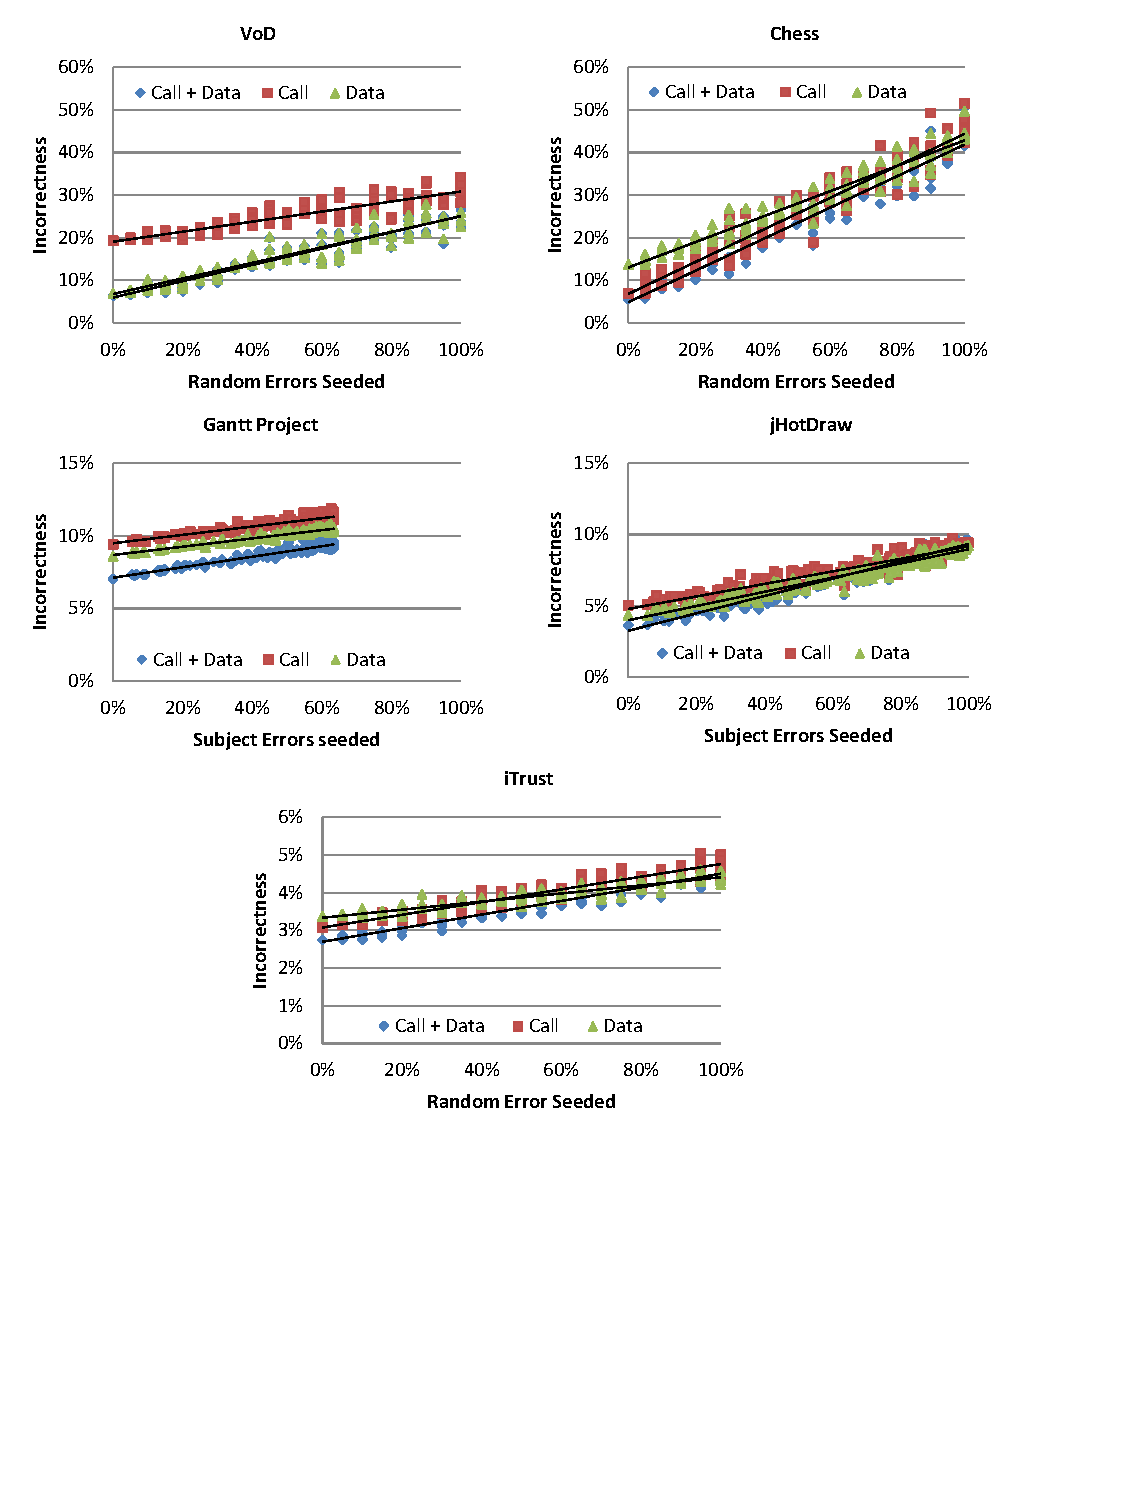
\includegraphics[width=5in]{FIGs/chapter4/errorExpCH4.pdf}
  \caption{以含错误的RTM为输入的五个系统上三个实验(Call,Data,Call+Data)的错误率(Incorrectness)}\label{fig_errorExpCH4}
\end{figure}

\textbf{注意:不要删除FIGs下面的njulogo和njuname这两个文件,这是论文封面的校徽和手写体南大校名。}

\section{引用代码}

\begin{figure}[htb]
  \centering
  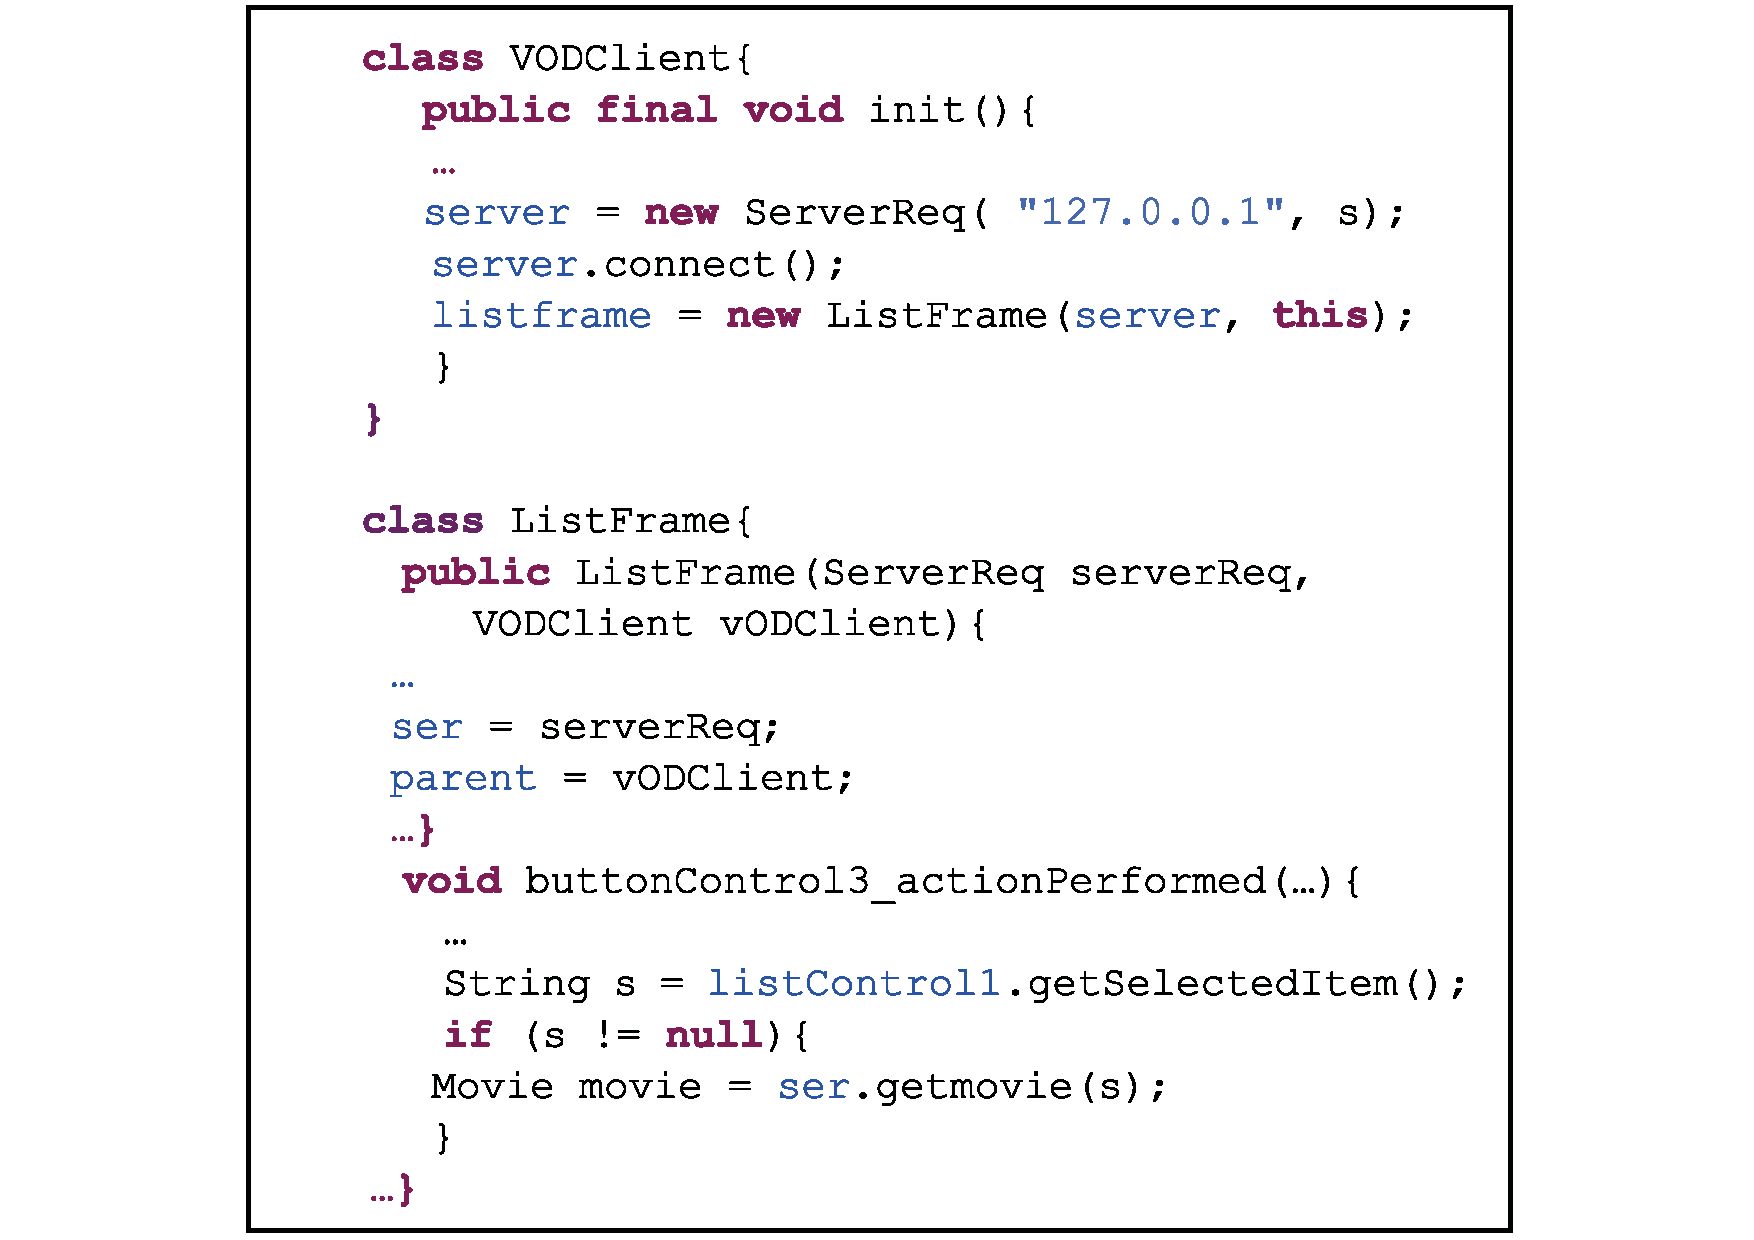
\includegraphics[width=\linewidth]{FIGs/chapter4/VoDCodeSample.pdf}
  \caption{VoD系统中的代码片段}\label{fig_VoDCodeSample}
\end{figure}

这里给出一个代码引用的推荐实践。
引用代码时先将代码放入word的文本框中,调整结束后,将该文本框页面另存为pdf文件,之后再作为图形来引用,如图~\ref{fig_VoDCodeSample}所示。




\chapter{公式}

这里直接给出几个较为复杂的公式的例子,可一一进行参照。
若有未包含的数学符号或公式格式,请参阅本模板所包含的手册(本地manual文件夹)或百度必应谷歌。

\section{公式5.1与论证}
“从直接代码依赖的角度出发,从一个初始域外的类$C_{out}$ 出发我们尝试找到一个通往初始域内的类$C_{in}$ 的路径。一条合法的路径需要满足以下两点要求:(1)这一路径是单向的,即$C_{out}$ 传递性地到达$C_{in}$ 或$C_{in}$ 传递性地到达$C_{out}$;(2)路径中只能包含一个$C_{in}$ (为了避免重复路径的出现)。为了恰当的估计一条合法路径所代表的交互程度,我们计算路径上所有直接代码依赖的紧密度值的几何平均。我们用如下公式来重新计算给定$C_{out}$ 的IR 值($IR_{DC}$):”

\begin{align}
IR_{DC}=IR_{origin}+(IR_{top}-IR_{origin})^{\left| PATH\right|}\sqrt {\prod _{x \in PATH}Closeness_{DC}(x)} \end{align}

“其中$IR_{origin}$ 代表$C_{out}$ 的初始IR值,$IR_{top}$ 代表$C_{in}$ 被提升过的IR值,\emph{PATH} 代表$C_{out}$ 与$C_{in}$ 之间的路径内所有的直接代码依赖,而$Closeness_{DC}(x)$ 则代表每一条直接代码依赖关系的紧密度值。在同一对$C_{out}$ 和$C_{in}$ 之间可能存在多条合法路径,我们只保留其中能使$IR_{DC}$ 值最大的那条路径。”

\section{公式5.2与论证}

“由于IR 方法返回的是一个按照IR 值大小倒序排列的候选线索列表,因此一种常用的比较IR 方法的方式是在不同的查全率水平上比较不同方法之间的精确度,通常用$Precision-Recall$ 曲线表示。为了进一步衡量IR 方法返回结果的整体质量,我们选用了另外两个常用的实验度量:$AP$(Average Precision)与$MAP$ (Mean Average Precision)。其中,$AP$ 用于度量全部查询(需求)所检索的相关文档的排序质量,计算方式如下:”
\begin{align}
AP=\dfrac {\sum _{r=1}^{N}\left( Precision\left( r\right) \times isRelevant\left( r\right) \right) } {\left| RelevantDocuments\right| }
\end{align}

“其中,$r$ 表示被查询对象(类)在列表中的排序,$Precision(r)$ 表示前$r$ 个类的准确率。$isRelevant()$ 为一个二值函数,如果文档是相关的,则返回1,若无关,则返回0。”

\section{公式5.3与论证}

“由此,我们为类数据依赖定义紧密度$Closeness_{CD}$ 如下:”

\begin{align}Closeness_{CD}=\frac {\sum _{x \in \{DT_{i}\cap DT_{j}\}}idtf(x)} {\sum _{y \in \{DT_{i}\cup DT_{j}\}}idtf(y)}\end{align}

“其中$idtf(x)$ 代表共享数据类型的idtf值,$DT_i$ 与$DT_j$ 的交集代表该数据依赖上的共享数据类型,而$DT_i$ 与$DT_j$ 的并集则代表$C_i$ 和$C_j$ 在全部代码上所访问的数据类型。$Closeness_{CD}$ 的取值范围是0到1之间。”


\chapter{算法}

同样是定义+引用的方式,参见算法~\ref{alg:Re-rankLinksOutsideInitialRegion}。
本算法已包含大量常用格式,如有未包含的数学符号或格式,请参阅本模板所包含的手册或询问百度必应谷歌。
如论文中无需算法则不用强加。

\begin{algorithm}[htbp]
\caption{初始需求域外追踪线索的重排}
\label{alg:Re-rankLinksOutsideInitialRegion}
topIRValue $\leftarrow$ initialRegion.topIRValue;\\
\ForEach {link in candidateList} {
  \If {!initialRegion.contains(link.class)} {
      \ForEach {c in initialRegion} {
          pathList $\leftarrow$ findValidPaths(link.class, c);\\
            $gMean$ $\leftarrow$ 0;\\
            \ForEach {path in pathList} {
              $gMean$ $\leftarrow$ max(GeometricMean($Closeness_{DC}$(path)), $gMean$);
            }
            link.IRValue $\leftarrow$ link.IRValue + $gMean$(topIRValue - link.IRValue);\\
            \If {hasDataDependencies(c, link.class)} {
              link.IRValue $\leftarrow$ link.IRValue + $Closeness_{CD}$(c, link.class)(topIRValue - link.IRValue);
            }
        }
        \If {link.IRValue \textgreater \ topIRValue} {
          link.IRValue $\leftarrow$ topIRValue;
        }
    }
}
candidateList.reorderByIRValue();
\end{algorithm}

\chapter{论文引用}

此处的论文引用采用的是类似于IEEE的按出现位置的数字编号格式。建议将被引用的论文全名放入dblp网站(必应谷歌搜索dblp)搜索,之后进入该论文详细信息,如图~\ref{fig_dblpForBibtexCH7} 所示。

\begin{figure}[htb]
  \centering
  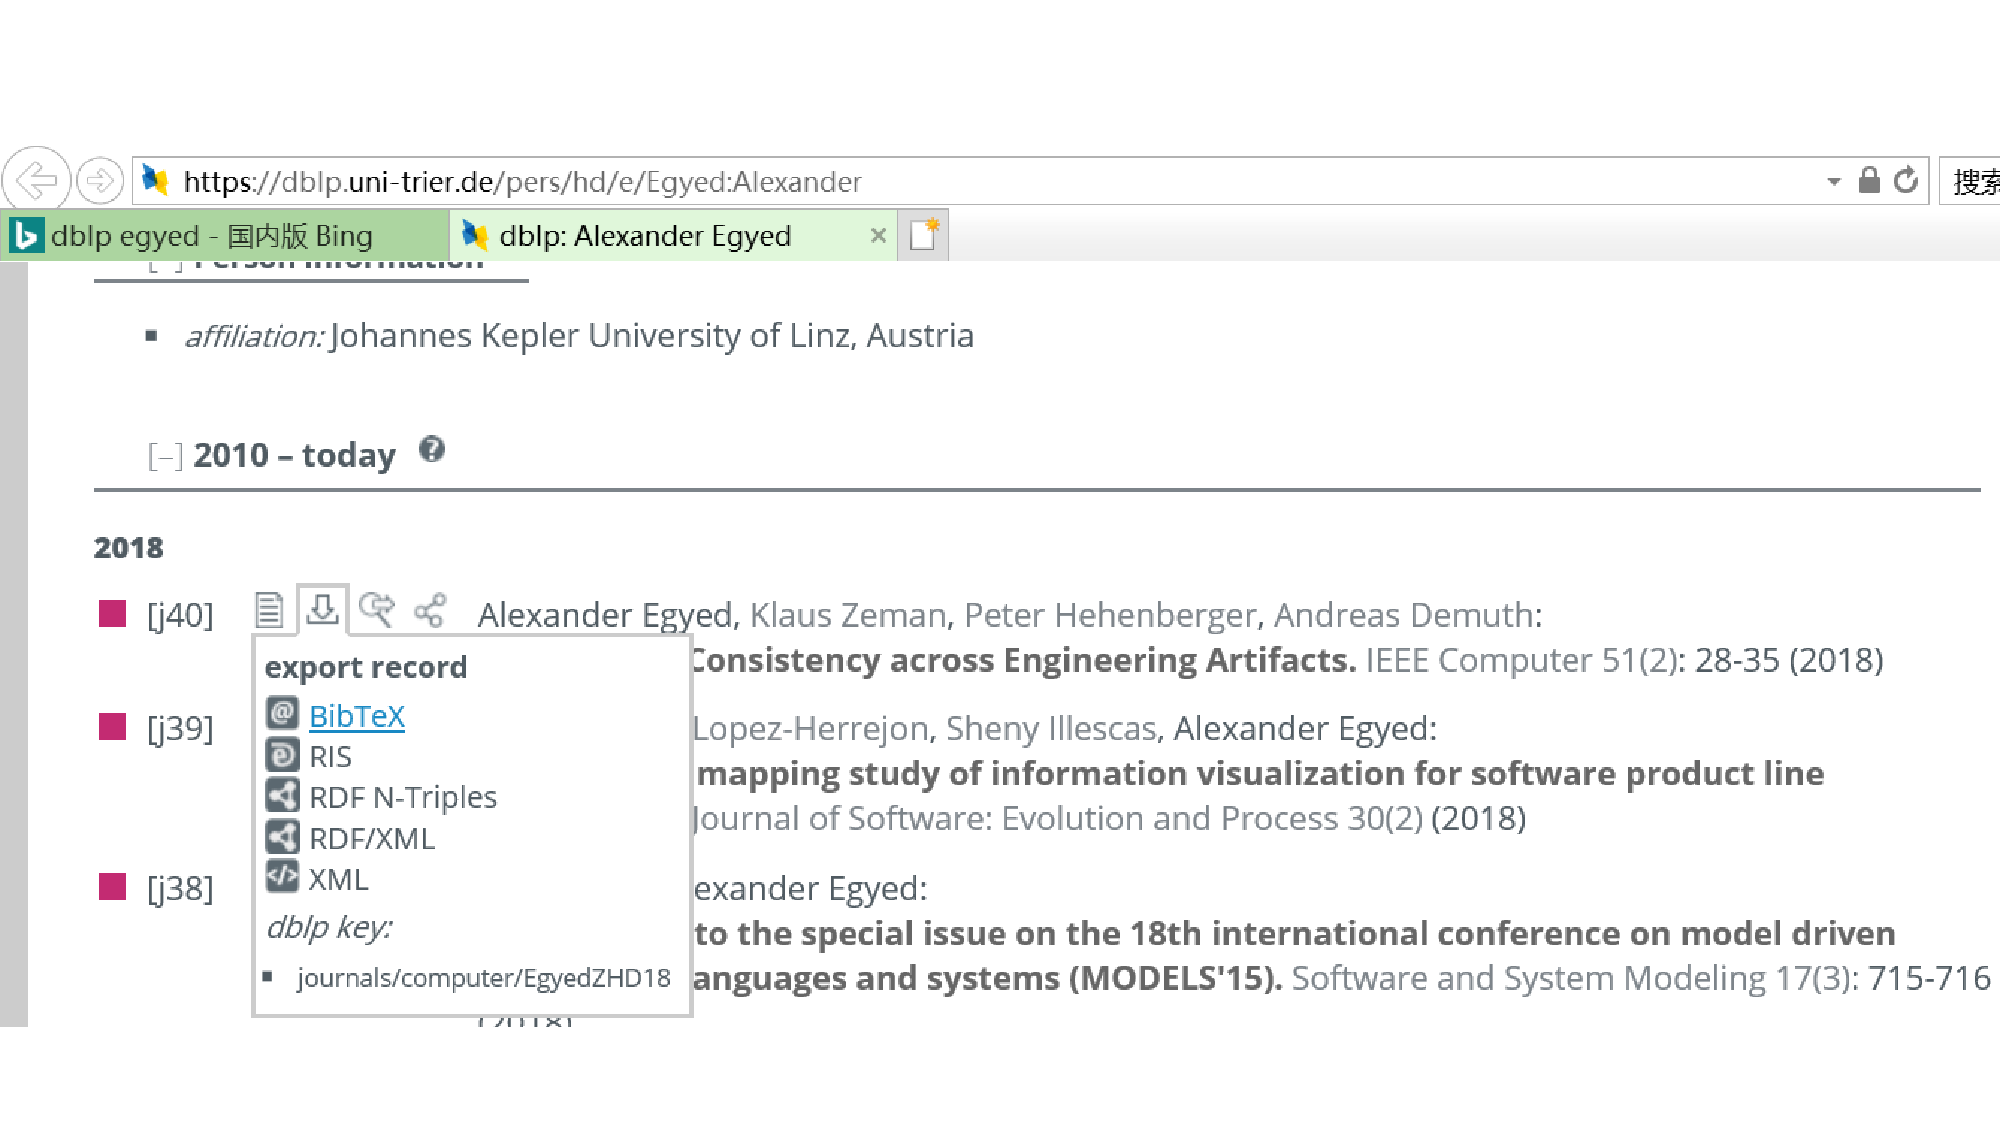
\includegraphics[width=5in]{FIGs/chapter7/dblpForBibtex.pdf}
  \caption{在dblp上下载Bibtex}\label{fig_dblpForBibtexCH7}
\end{figure}

点击该链接之后将得到Bibtex信息,如图~\ref{fig_bibtexDetailCH7}所示。
打开本地文件夹下的reference.bib文件,完整添加该信息。
并在需要引用的位置添加这一引用~\cite{DBLP:journals/computer/EgyedZHD18}。
格式为bibtex信息中的开头,\emph{例如图中的“DBLP:journals/computer/EgyedZHD18”。(此处是一个典型的因为长字符串导致的bad box,请参考上述章节的内容手动完整软换行)}。

\textbf{注意:在修改并保存reference.bib文件后,先点击PDFLaTeX旁边的B按钮编译bib文件,之后需要连续使用PDFLaTeX编译两次,直到最后控制台输出的Warnings不再增加,此时才完成一次论文引用的更新。}

在bib文件中出现,但并未在论文中被引用的论文不会出现在最后的参考文献中。如果dblp中并未包含你需要的论文,则可以尝试谷歌或百度学术的搜索结果,一般也包含bibtex信息,但可能不完整或不规范。

引用网站链接可以考虑这一格式~\cite{GanttSystem}(不推荐,网站链接使用脚注更规范些)。

引用书籍可以考虑这一格式~\cite{Pohl2010Requirements}。

中文文献请参考这一格式~\cite{cyg2006}(引用标记请避免中文,否则容易出现编译错误)。

以下英文引用用来测试引文排序是否按照插入顺序,以及多引文是否合并~\cite{DBLP:journals/computer/EgyedZHD18, DBLP:journals/ml/TingZCZWZ19}

\begin{figure}[htb]
  \centering
  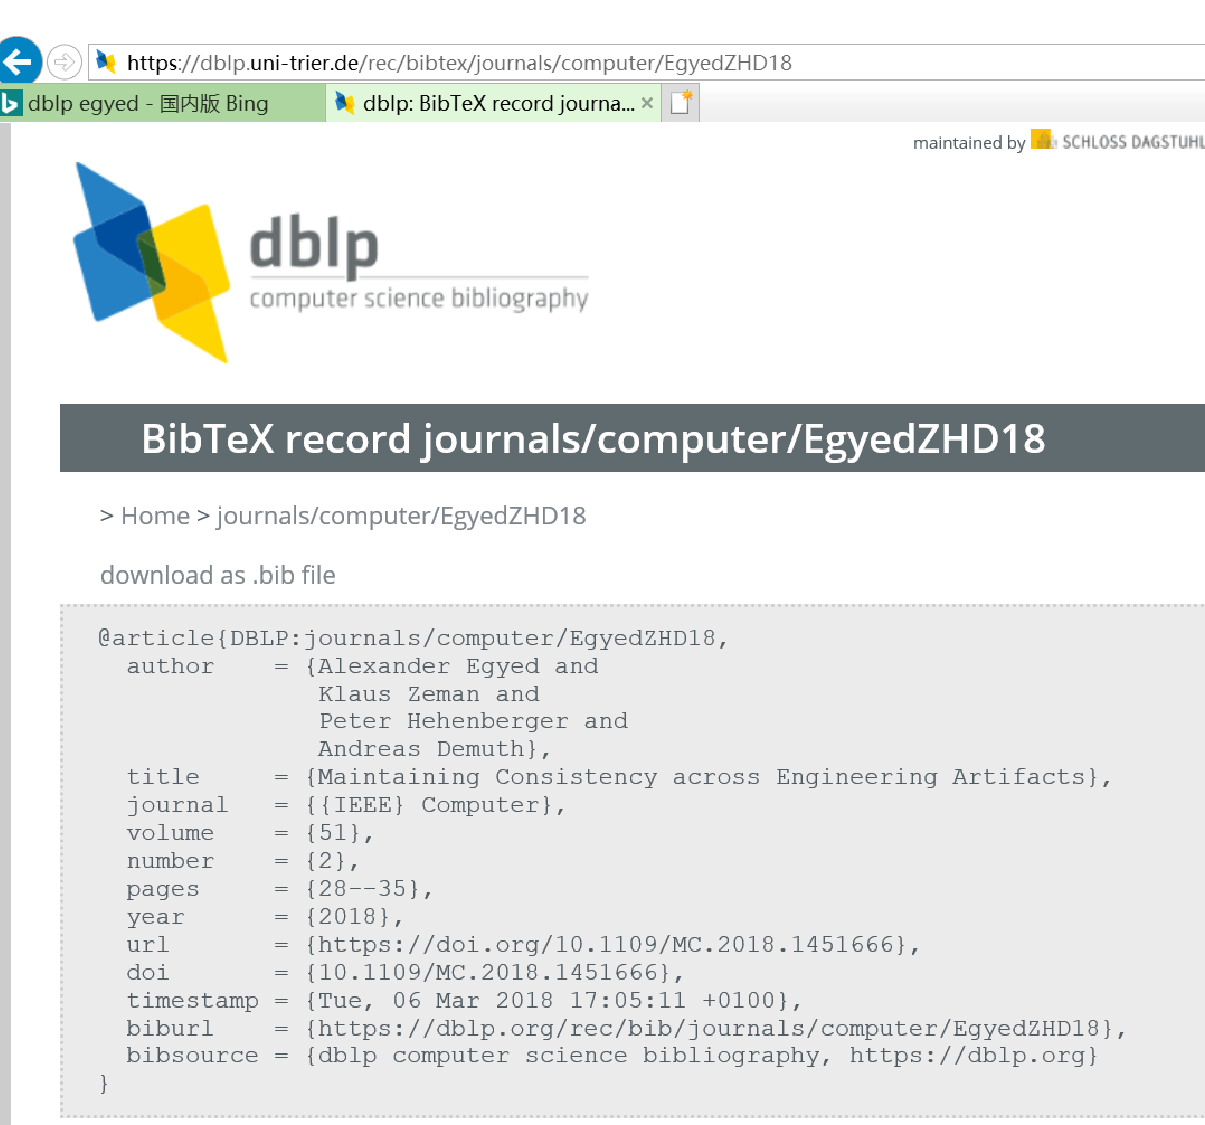
\includegraphics[width=5in]{FIGs/chapter7/bibtexDetail.pdf}
  \caption{Bibtex详细信息}\label{fig_bibtexDetailCH7}
\end{figure}


% 参考文献

\bibliography{reference}
%% addde by lhy
%% 因为overleaf上没有这个参考文献排版文件
% \bibstyle{elsart-num}


%个人简介
\Nchapter{简历与科研成果}
\noindent {\heiti 基本情况}
\vspace{1ex}
\noindent 徐文远,男,汉族,1995~年~8~月出生,江苏省南京市人。
\vspace{2ex}

\noindent {\heiti 教育背景}
\begin{description}[labelindent=0em, leftmargin=8em, style=sameline]
\item[2018.9~2020.6] 南京大学软件学院 \hfill 硕士
\item[2014.9~2018.6] 扬州大学信息工程学院 \hfill 本科
\end{description}
% 发表文章目录

\noindent {\heiti 这里是读研期间的成果(实例为受理的专利)}

\begin{enumerate}[label=\arabic*., labelindent=0em, leftmargin=*]
	\item 李四,\textbf{张三},``一种使用Hammer砸碎Nut的方法'',申请号:20xx1018xywz.a,已受理。
\end{enumerate}


\backmatter


\begin{thanks}

\vskip 18pt

这里是致谢。
一般的感谢顺序:导师,其他指导老师,师兄弟姐妹、同学,父母和伴侣。

\end{thanks}


\end{document}


